% Лекции Сергея Борисовича Стечкина
% Внесены исправления В.В.Арестова, версия 06.07.2009
% Внесены исправления Н.И.Черныха, версия 29.07.2009
% Внесена грамматическая и ТеХ-правка М.Дейкаловой, версия 05.08.09

 %%%%%%%%%%%%%%%%%%%%%%%%%%%%%
 \chapter{Нормы сумм Валле Пуссена (продолжение)}
 %%{Лекция 17.}

 \section{Доказательство теоремы Никольского}


Докажем  теорему Никольского, сформулированную в конце предыдущей лекции. Суммы
 Валле Пуссена%\footnote{{В обозначениях,
% принятых в лекции~\ref{ch6}, нынешняя $\sigma_{n,p}$ обозначалась бы $\sigma_{n,n-p}$,
% что следует помнить при} {использовании результатов из этой лекции.}}
 \ $\sigma_{n,p}$  представляются  через суммы Фейера $\sigma_n$:
 %\Green{Николай Иванович хочет, чтобы текст из скобок был сделан в виде сноски внизу страницы.}:
  $$
 \sigma_{n,p}(f)=\frac{1}{p+1} \sum\limits_{k=n-p}^n s_k(f)=\frac{n+1}{p+1}
 \sigma_n(f)-\frac{n-p}{p+1} \sigma_{n-p-1}(f);
 $$
 в случае  $p=n$ считаем, что  $\sigma_{n-p-1}(f)=\sigma_{-1}(f)\equiv 0.$
 Для сумм Фейера известно интегральное представление (см. параграф~\ref{s5-2})
 $$
 \sigma_{n}(f)=\sigma_{n,n}(f)=
 \frac{1}{2\pi(n+1)} \int_0^{2\pi} f(x+t)\left( \frac{\sin
 \frac{n+1}{2}\,t}{\sin \frac{t}{2}}\right)^2\, dt.
 $$
 В результате для сумм Валле Пуссена получаем представление
 $$
 \sigma_{n,p}(f)=
 \frac{1}{2\pi(p+1)} \int_0^{2\pi} f(x+t)\left\{
 \left( \frac{\sin \frac{n+1}{2}\,t}{\sin \frac{t}{2}}\right)^2-
 \left( \frac{\sin \frac{n-p}{2}\,t}{\sin \frac{t}{2}}\right)^2\right\}\,
 dt=
 $$
 $$
 =\frac{1}{\pi(p+1)} \int_0^{2\pi} f(x+t)
 \frac{\sin \frac{2n+1-p}{2}\,t\cdot \sin \frac{p+1}{2}\,t}
 {2\sin^2 \frac{t}{2}}\, dt,
 $$
 т.\,е.
 $$
 \sigma_{n,p}(f)=\int_0^{2\pi} f(x+t)K(t)\, dt,\ \ \mbox{где}\ \  K(t)=\frac{1}{\pi(p+1)} \cdot
 \frac{\sin \frac{2n+1-p}{2}\,t\cdot \sin \frac{p+1}{2}\,t}
 {2\sin^2 \frac{t}{2}}.
 $$
Итак, суммы Валле Пуссена являются оператором свертки
 с непрерывным ядром  $K.$
 Норма такого оператора в пространстве $C,$ как мы знаем, вычисляется по формуле
 $$
 \|\sigma_{n,p}\|=\|\sigma_{n,p}\|_C^C=\int_0^{2\pi} |K(t)|\, dt.
 $$
Ядро $K$ является четным, поэтому
 $$
 \|\sigma_{n,p}\|=2\int_0^{\pi} |K(t)|\, dt=
 \frac{2}{\pi(p+1)} \int_0^{\pi}
 \left| \frac{\sin \frac{2n+1-p}{2}\,t\cdot \sin\frac{p+1}{2}\,t}
 {2\sin^2\frac{t}{2}} \right|\, dt.
 $$

Задача свелась к исследованию последнего интеграла. Введем обозначения
 $$
 m=\dfrac{p+1}{2},\qquad r=\dfrac{2n+1-p}{p+1};
 $$
 имеем $m\ge \dfrac{1}{2}$,~
$r\ge 1.$ Отметим, что $rm=\dfrac{2n+1-p}{2}.$
 В этих обозначениях
 $$
 \|\sigma_{n,p}\|=\frac{1}{\pi m}\int_0^{\pi}
\frac{ \left| \sin rmt\cdot \sin mt \right|}
 {2\sin^2\frac{t}{2}}\, dt.
 $$
 Так как
 $$
 \frac{1}{\sin^2 \frac{t}{2}}-\frac{4}{t^2}=O(1),\qquad 0<t\le\pi,
 $$
 и числитель выражения под знаком интеграла ограничен, можно записать
 $$
 \|\sigma_{n,p}\|=\frac{2}{\pi m}\int_0^{\pi}
 \frac{|\sin rmt\cdot \sin mt|}
 {t^2}\, dt+O\left( \frac{1}{m} \right)=
 $$
 $$
 =\frac{2}{\pi m}\int_0^{\pi}
 \frac{|\sin rmt\cdot \sin mt|}
 {t^2}\, dt+O(1).
 $$
 Введем новую переменную  $u=mt.$ Тогда последнее выражение примет вид
 $$
 \frac{2}{\pi}\int_0^{\pi m}
 \frac{|\sin ru\cdot \sin u|}
 {u^2}\ du+O(1).
 $$
 Поскольку  $\displaystyle\int_{\pi}^{\infty}\frac{du}{u^2}=O(1),$ то
  $$
 \frac{2}{\pi}\int_0^{\pi m}
 \frac{|\sin ru\cdot \sin u|}
 {u^2}\ du= \frac{2}{\pi}\int_0^{\pi}
 \frac{|\sin ru\cdot \sin u|}
 {u^2}\ du+O(1).
 $$
 Далее, в силу соотношения
 $$
 \frac{\sin u}{u^2}-\frac{1}{u}=O(1),\qquad u\in (0,\pi],$$
имеем
 $$
 \|\sigma_{n,p}\|=\frac{2}{\pi} \int_0^{\pi} \frac{|\sin ru \cdot \sin
 u|}{u^2}\ du+O(1)
 =\frac{2}{\pi} \int_0^{\pi} \frac{|\sin ru|}{u}\ du+O(1).
 $$
 Применяя теперь утверждение леммы~\ref{l16-1a}, получаем
  $$
 \|\sigma_{n,p}\|=
 \frac{4}{\pi^2} \ln r+O(1).
 $$
 Поскольку  $ 0\le p\le n,$ то  $n+1\le 2n+1-p\le 2n+1.$  Как следствие,  $2n+1-p \asymp n$ и
 $$
 \ln(2n+1-p)=\ln n+O(1).
 $$
Окончательно для норм сумм Валле Пуссена имеем
 $$
 \|\sigma_{n,p}\|_C^C=\frac{4}{\pi^2}\ln \frac{n}{p+1}+O(1).
 $$
 Теорема доказана.


 \begin{Remark} %%%   Замечание.
 Пусть $H$ --- однородное пространство (см. замечание~\ref{r16-1}), т.\,е.
 банахово пространство $2\pi$-периодических суммируемых функций со свойствами
 $\|f(x+h)\|_H=\|f(x)\|_H,$~ $h\in (-\infty,\infty),$ и $\|\Delta_h f\|_H\to 0,$~
 $h\to 0,$ для любой функции $f\in H.$
 В этом случае
 $$
 \|\sigma_{n,p}(f)\|_H=\left\| \int_0^{2\pi} f(x+t)K(t)\, dt
 \right\|_H\le
 $$
 $$
 \le \int_0^{2\pi} |K(t)| \|f(x+t)\|_H\, dt= \|f\|_H
 \int_0^{2\pi} |K(t)|\, dt \qquad \forall\ f\in H,
 $$
 т.\,е.
 $$
 \|\sigma_{n,p}\|_H=\|\sigma_{n,p}\|_H^H\le \int_0^{2\pi} |K(t)|\, dt=
 \|\sigma_{n,p}\|_C.
 $$
 Вот почему важен случай пространства  $C.$
 \end{Remark}

 \begin{Corollary} При $1\le q<\infty$
\begin{equation}\label{17-1}
 \|\sigma_{n,p}\|_{L_q}=\|\sigma_{n,p}\|_{L_q}^{L_q}\le
 \frac{4}{\pi^2}\ln \frac{n}{p+1}+O(1).
 \end{equation}
 \end{Corollary}

 При $q=1$ на самом деле здесь имеет место равенство, а при $1<q<\infty$
 оценка верна, но уже не точна.


 \section{Приложение сумм Валле Пуссена \\ к приближению непрерывных
 функций}

 Для натурального числа $k$ обозначим через   ${C}^{(k)}={C}^{(k)}_{2\pi}$
 множество $k$ раз непрерывно дифференцируемых (на всей числовой оси)
 $2\pi$-периодических функций.



 \task %%% Задача.
 Для функции $f\in {C}^{(k)} $ и тригонометрического полинома $t_n$
 известна норма  уклонения $\|f-t_n\|_C.$
 Как оценить $\|f^{(k)}-t_n^{(k)}\|_C?$


Следующая теорема содержит один из возможных ответов.

 \begin{teo}[о дифференцировании приближающих полиномов]\label{t17-1}
 Существует константа $A_k$ такая, что для каждой функции $f\in {C}^{(k)}_{2\pi} $ и любого
 тригонометрического полинома $t_n$ имеет место неравенство
 $$
 \|f^{(k)}-t_n^{(k)}\|_C\le A_k \left\{ n^k \|f-t_n\|_C+E_n
 (f^{(k)})_C\right\}.
 $$
 \end{teo}

 \begin{Corollary} %%% Следствие.
 Если $f\in C^{(k)}_{2\pi}$ и $n^k \|f-t_n\|_C\to 0$~ $(n\to \infty),$ то
 $\|f^{(k)}-t_n^{(k)}\|_C\to 0$ $(n\to \infty).$
 \end{Corollary}

  \begin{Remark} %%% Замечание.
 Одного условия $\|f-t_n\|_C=o(n^{-k})$
 недостаточно для того, чтобы утверждать, что $f\in {C}^{(k)}.$
 \end{Remark}

 \begin{Remark} %%% Замечание.
 Эти утверждения верны и в пространствах $L^p=L^p_{2\pi},$ $1\le p<\infty,$
 так как при доказательстве теоремы~\ref{t17-1} будут использоваться только
 суммы Валле Пуссена, свойство~(\ref{17-1}) этих сумм и
 неравенство Бернштейна (в случае $C_{2\pi}$ усиленное в следующей
 лемме).
 \end{Remark}



 \begin{lemma}[обобщенное неравенство Бернштейна, {С.\,Б.\,Стечкин, 1948 г.}]\label{l17-1}
 Для произвольного  тригонометрического полинома $t_n$ порядка $n$ справедливы
 неравенства
 $$
 \|t_n'\|_C\le \frac{n}{2\sin \frac{nh}{2}} \|\Delta_h t_n\|_C,\qquad
 0<h<\frac{2\pi}{n},
 $$
 и, как следствие, неравенства
 $$
 \|t_n^{(k)}\|_C\le \Big(\frac{n}{2\sin \frac{nh}{2}}\Big)^{k} \|\Delta_h^k t_n\|_C,\qquad
 k\in \mathbb N.
 $$
\end{lemma}

Положив в последних неравенствах $h=\dfrac{\pi}{n}$ и
учитывая, что $\|\Delta^kf(x)\|_C\le 2^k\|f\|_C,$
 получим классическое неравенство  Бернштейна
\begin{equation}\label{17-2}
 \|t_n'\|_C\le \frac{n}{2} \|\Delta_{\frac{\pi}{n}} t_n\|_C \le
 n\|t_n\|_C
\end{equation}
и его следствие
$$
\|t_n^{(k)}\|_C\le n^k \|t_n\|_C.
$$


 Д\;о\;к\;а\;з\;а\;т\;е\;л\;ь\;с\;т\;в\;о\quad  леммы~\ref{l17-1}. Пусть $x_0$ есть точка,
 в которой достигается максимум $|t_n'|;$ предположим для определенности, что
 $t_n'(x_0)>0.$ Обозначим
 $$
 M_1= \max |t_n'(x)|=t_n'(x_0).
 $$
 Определим  функцию сравнения
 $$
 \varphi_n(x)= \varphi_n(x,t_n)=M_1\cos n(x-x_0).
 $$




 %%%%%%%%%%%%%%%%%%%%%%%%%%%%%%%%%%%%%%%%%%%%%%%%%%%%%%
% \hbox to 0.5cm {}{\special{em:graph pict1.pcx}}
% \vspace{6cm}
 %%%%%%%%%%%%%%%%%%%%%%%%%%%%%%%%%%%%%%%%%%%%%%%%%%%%%%%%%%
\begin{figure}[ht]
\begin{center}
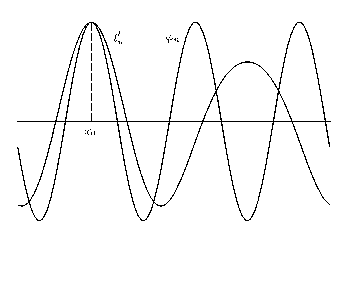
\includegraphics[width=0.5\textwidth]{pict17-1.eps}
\end{center}
 \refstepcounter{ris}\label{r17-1}
 \centerline{Рис.~\theris}
\end{figure}

 \noindent
 Рассмотрим отрезок $\left[ x_0-\dfrac{\pi}{n}, x_0+\dfrac{\pi}{n}
 \right]=I,$ являющийся одним из наименьших периодов функции $\varphi_n.$
 Оказывается (см. рис.~\ref{r17-1}), что
$$
 \varphi_n(x)\le t_n'(x)\qquad \forall\ x\in
 \left[ x_0-\frac{\pi}{n}, x_0+\frac{\pi}{n}\right]=I.
$$
 Докажем это свойство рассуждениями  от противного. Предположим, что существует точка $x'\in I,$
 в которой $t_n'(x')< \varphi_n(x').$ {Тогда на промежутке $I$ кроме $x_0$ найдется}
{по крайней мере еще один нуль $x''$ функции
$t_n'-\varphi_n$ {(см. рис.~\ref{r17-2}).}}

\begin{figure}[ht]
\begin{center}
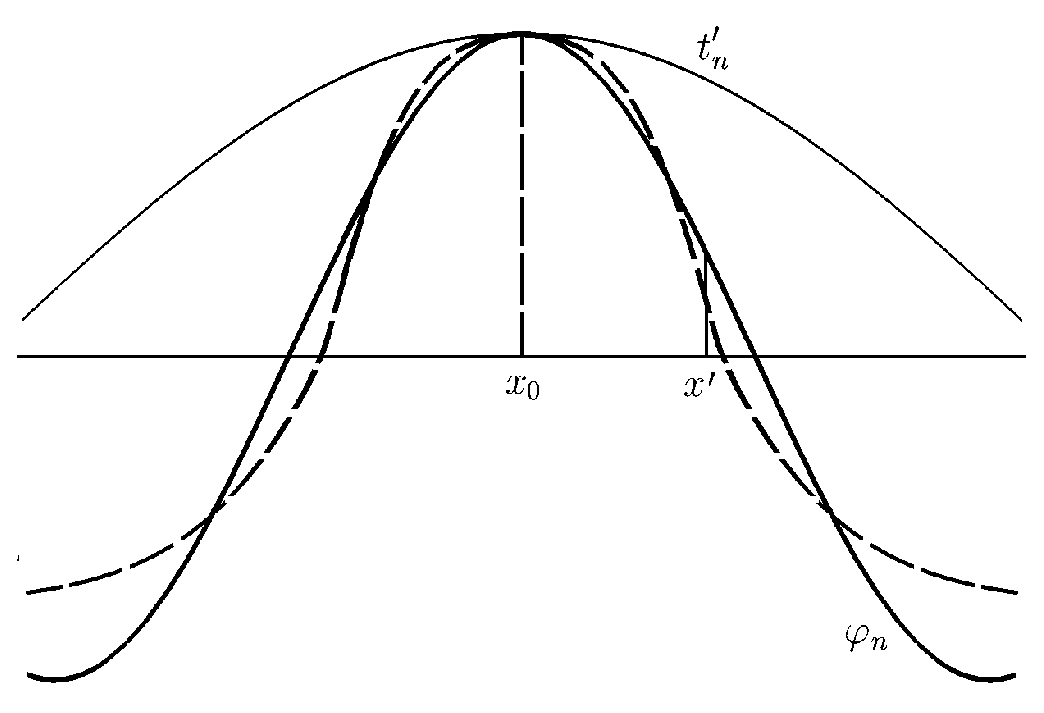
\includegraphics[width=0.5\textwidth]{pict17-2.eps}
\end{center}
% \bigskip
 \refstepcounter{ris}\label{r17-2}

\centerline{Рис.~\theris}
\end{figure}

%\bigskip

% \noindent
 Будем считать нули разности $t_n'-\varphi_n.$  Рассмотрим отрезки, на которых
 $\cos n(x-x_0)$ один раз
 меняется от $-1$ до 1. На каждом из этих отрезков график $\varphi_n$
 пересекается с графиком  $t_n';$
 при этом, если пересечение осуществляется  в точке экстремума $\varphi_n$, то  эта
 точка является двойным корнем разности  $t_n'-\varphi_n.$ С учетом кратностей, график
 полинома $\varphi_n(x)=M_1 \cos n(x-x_0)$
 пересекает график  $t_n'$ {по крайней мере} столько раз, сколько $\cos n(x-x_0)$
 изменяется от $-1$ до 1. Таким образом, вне основного
 отрезка $I$ имеется $2n-2$ нуля разности $t_n'-\varphi_n,$
 {если она не зануляется в концах отрезка $I$;} кроме того,  на $I$
существуют еще два нуля -- в точке $x_0$ (двойной нуль) и в точке {$x''\in {\rm int}\, I$}
 (по предположению). Таким образом, при сделанном дополнительном предположении
 всего на периоде разность $t_n'-\varphi_n$ имеет
 (с учетом кратности), по крайней мере $2n-2+2+1=(2n+1)$
 нулей. {Ясно, что если $x''$ совпадает с одним из концов отрезка $I$ или
 функция $t_n'-\varphi_n$}
 {зануляется в обоих его концах, то общее число ее нулей на периоде
 не уменьшится.}  Однако  $t_n'-\varphi_n$ есть (ненулевой)  тригонометрический
 полином порядка $n$
 и не может иметь столько нулей  (на периоде). Пришли к противоречию. Значит,
 действительно, справедливо неравенство
 $$
 M_1\cos n(x-x_0)\le t_n'(x)\qquad \forall\ x\in
 \left[ x_0-\frac{\pi}{n},x_0+\frac{\pi}{n} \right].
 $$

 Проинтегрируем последнее неравенство по $x$ на
 $ \left[ x_0-\dfrac{h}{2},x_0+\dfrac{h}{2} \right]\subset I$
 при $0<h<\dfrac{2\pi}{n}.$ В результате получим
 $$
 M_1 \int_{x_0-\frac{h}{2}}^{x_0+\frac{h}{2}}\cos n(x-x_0)\, dx=
 \frac{M_1}{n} 2\sin \frac{nh}{2}\le
 $$
 $$
 \le \int_{x_0-\frac{h}{2}}^{x_0+\frac{h}{2}} t_n'(x)\, dx=
 t_n\left(x_0+\frac{h}{2}\right)- t_n\left(x_0-\frac{h}{2}\right)\le
 \|\Delta_ht_n\|_C
 $$
 и, так как $M_1=\|t_n'\|_C,$ то лемма при $k=1$ доказана.
 Пусть при $0<h<\dfrac{2\pi}{n}$ верно неравенство
 $$
 \|t_n^{(k-1)}\|\le \bigg( \dfrac{n}{2\sin\frac{nh}{2}}\bigg)^{k-1}\|\Delta_h^{k-1}
 t_n\|_C.
 $$
 Тогда при $0<h'<\dfrac{2\pi}{n}$ по доказанному
 неравенству
 $$\|t_n^{(k)}\|_C\le \dfrac{n}{2\sin\frac{nh'}{2}}\|\Delta_{h'} t_n^{(k-1)}\|_C=
\bigg(
\dfrac{n}{2\sin\frac{nh'}{2}}\bigg)\|(\Delta_{h'}
t_n)^{(k-1)}\|_C\le
$$
$$
\le \bigg( \dfrac{n}{2\sin\frac{nh'}{2}}\bigg)
\left( \dfrac{n}{2\sin nh}\right)^{k-1}\|\Delta_h^{k-1}(\Delta_{h'} t_n)\|.
$$
Полагая теперь $h'=h\in \Big(0,\dfrac{2\pi}{n}\Big),$
получим требуемое

%\newpage
 Д\;о\;к\;а\;з\;а\;т\;е\;л\;ь\;с\;т\;в\;о\quad теоремы~\ref{t17-1}.
 Представим разность $f-t_n$ в виде
 $$
 f-t_n=f-\sigma_{n+p,p}(f)-(t_n-\sigma_{n+p,p}(f)).
 $$
 Продифференцируем это тождество $k$ раз:
 $$
 f^{(k)}-t_n^{(k)}=f^{(k)}-\sigma_{n+p,p}(f^{(k)})-(t_n-
 \sigma_{n+p,p}(f))^{(k)}.
 $$
Отсюда получаем
 $$
 \|f^{(k)}-t_n^{(k)}\|_C\le \|f^{(k)}-\sigma_{n+p,p}(f^{(k)})\|_C+\|(t_n-
 \sigma_{n+p,p}(f))^{(k)}\|_C.
 $$
 Применяя неравенство Лебега  (для метода Валле Пуссена), имеем
 $$
 \|f^{(k)}-\sigma_{n+p,p}(f^{(k)})\|_C\le
 ({\|\sigma_{n+p,p}\|_C^C}+1) E_n(f^{(k)})_C.
 $$
 Далее, применяя неравенство Бернштейна и вновь неравенство  Лебега, получаем
 $$
 \|(t_n-
 \sigma_{n+p,p}(f))^{(k)}\|_C\le (n+p)^k \|t_n-
 \sigma_{n+p,p}(f)\|_C\le
 $$
 $$
 \le
  (n+p)^k (\|f-t_n\|_C+\|f-
 \sigma_{n+p,p}(f)\|_C)
 \le
 $$
 $$
 \le (n+p)^k \left\{
 \|f-t_n\|_C+({\|\sigma_{n+p,p}\|_C^C}+1)\|f-t_n\|_C\right\} =
 $$
 $$
 =({\|\sigma_{n+p,p}\|_C^C}+2)  (n+p)^k
 \|f-t_n\|_C.
 $$
 Таким образом,  справедливо неравенство
 \begin{equation}\label{f17-1}
 \|f^{(k)}-t_n^{(k)}\|_C\le (\|\sigma_{n+p,p}\|_C+2) \left\{ (n+p)^k
 \|f-t_n\|_C+E_n(f^{(k)})_C\right\}. %\eqno(1)
 \end{equation}

 Положим здесь $p=n.$ По  теореме Никольского нормы $\|\sigma_{2n,n}\|$
 ограничены (по $n$). Поэтому  из {\eqref{f17-1}} следует оценка
 $$
 \|f^{(k)}-t_n^{(k)}\|_C\le A_k \left\{ n^k \|f-t_n\|_C+E_n
 (f^{(k)})_{{C}}\right\}.
 $$
 Теорема доказана.

 \begin{Remark} %%%Замечание.
 Приведенное  доказательство дает значение $A_k=O(2^k).$ На самом деле можно получить   $A_k=O(\ln(k+1)).$
 Для обоснования этого необходимо   надлежащим образом выбрать
 параметр $p.$ Из оценки {\eqref{f17-1}}  по теореме
 Никольского получим
 $$
 \|f^{(k)}-t_n^{(k)}\|_C\le \left\{ \frac{4}{\pi^2}\ln
 \frac{n+p}{p+1}+O(1) \right\} \left( \frac{n+p}{n}\right)^k \left(
 n^k \|f-t_n\|_C+E_n (f^{(k)})_C\right).
 $$
 Путем выбора $p=p(n)$ сделаем величину
  \begin{equation}\label{f17-2}
\left\{ \frac{4}{\pi^2}\ln \frac{n+p}{p+1}+O(1)\right\} \left(
 \frac{n+p}{n}\right)^k %\eqno(2)
  \end{equation}
 как можно меньше. Рассмотрим два случая.

 {\Case $k\le n.$} Выберем целое $p$ так, чтобы $\dfrac{n}{k}-1\le p\le \dfrac{n}{k}.$
 Тогда
 $$
 \left( \frac{n+p}{n}\right)^k \le \left( 1+
 \frac{{n}/{k}}{n}\right)^k = \left(
 1+\frac{1}{k}\right)^k\le e,
 $$
 $$
 \frac{n+p}{p+1}=\frac{n-1}{p+1}+1\le k\frac{n-1}{n}+1< k+1.
 $$
 При таком выборе параметра $p$ величина {$\eqref{f17-2}$}
 будет иметь значение   $O(\ln(k+1)),$ т.\,е. $A_k=O(\ln(k+1)).$

 {\Case $k\ge n.$}
 \noindent  Положим $p=0.$ В этом случае для величины {$\eqref{f17-2}$}  имеем {оценку}
 $$
 \frac{4}{\pi^2} \ln (n+1)+O(1)\le
 \frac{4}{\pi^2} \ln (k+1)+O(1)=O(\ln(k+1)).
 $$
 Итак, в обоих случаях получаем
 $$
 A_k=O(\ln(k+1)).
 $$
 \end{Remark}

 \task %%% Задача.
 Доказать, что этот порядок величины $A_k$ является точным.

 \begin{Remark} %%%Замечание.
 Неравенство Бернштейна~(\ref{17-2}) доказано нами в пространстве $C_{2\pi}.$
 Однако, как можно показать, оно имеет место и в любом однородном пространстве. Поэтому и
 теорема~\ref{t17-1} о дифференцировании приближающих полиномов
 верна не только в $C,$ но и в любом однородном пространстве (см. замечание в конце п.~17.1).
 \end{Remark}
